\documentclass{article}

\usepackage{verbatim}
\usepackage{amsthm}
\usepackage{amsfonts}
\usepackage{cleveref}


\usepackage{graphicx}

\newcommand{\Code}[1]{\texttt{#1}}
\newcommand{\Config}[2]{\ensuremath{\langle #1, #2 \rangle}}
\newcommand{\Rule}[2]{\ensuremath{#1 \hookrightarrow #2}}
\newcommand{\Trans}[3]{\ensuremath{#1 \rightarrow_{#2} #3}}
\newcommand{\Frame}[2]{[#1, #2]}

\newcommand{\powerset}[1]{P(#1)}
\newcommand{\epspath}[3]{\ensuremath{#1 to #2 via #3}}
\newcommand{\subsubsubsection}[1]{\textbf{#1}}
\newcommand{\bbN}{\mathbb{N}}
\newcommand{\meet}{\sqcap}
\newcommand{\extend}{\otimes}
\newcommand{\combine}{\oplus}

\newtheorem{definition}{Definition}
\newtheorem{example}{Example}

\newcommand{\poststar}{\ensuremath{\textsc{post}^\textsc{*}}}
\newcommand{\prestar}{\ensuremath{\textsc{pre}^\textsc{*}}}

\newcommand{\Zero}{\ensuremath{\overline{0}}}
\newcommand{\One}{\ensuremath{\overline{1}}}

\newenvironment{sidebar}{}{}

\newcommand{\strong}[1]{\textbf{#1}}

\begin{document}

This document will work up to a description of WPDSs as they are used
in program analysis. We will start with unweighted pushdown systems,
discussing their applications primarily in terms of verifying Boolean
programs, then move on to the weighted versions. In order to set the
stage for describing unweighted PDSs, we start with describing boolean
programs and use that as a launching point for discussing trasition
systems, which PDSs define.

In program analysis, pushdown systems are all about solving
\emph{reachability} problems. Unweighted PDSs can be used to answer
questions such as ``is this particular state reachable from the start
state?'' (For instance, perhaps you want to determine whether it is
possible for a program to reach an error state.) Weighted pushdown
systems are used to answer questions such as ``what is the net effect
on the program dataflow between the initial state and this particular
state?'' The latter question, if you tilt your head sideways, is just
another question about reachability.


\section{Boolean Programs}
The definition of a Boolean program is very simple: a Boolean program
is just a program where every variable has type Bool.

I will defer the question of why Boolean programs are useful for a
moment, and instead concentrate on their semantics. I'm going to leave
details of how the semantics are specified (e.g. small/large-step
operational, denotational, etc.) aside. What we're really interested
in at the moment is the \emph{structure of states} and \emph{which
  states are successors} of which other states; how you actually
determine the successor relation is less relevant.

In addition to the restriction that all variables are of type Bool,
here are some perhaps-unusual characteristics of Boolean programs:

\begin{itemize}
  \item 
    Boolean programs are allowed to have nondeterministic branches,
    notated as \Code{if(*)}. Both branches of such a branch are
    \emph{reachable}; this means that if you are trying to determine
    whether an error point is reachable, it can be located in either
    branch (or rely on variable settings from either branch). It is
    possible to use a nondeterministic branch for a loop as well,
    \Code{while(*)}.

  \item
    Boolean programs can have a \Code{assert} statements, which mark
    error points. Assertions don't have attached conditions, but such
    conditions can of course be simulated as
    \Code{if(I\_am\_having\_a\_bad\_day) \{ assert; \}}.


  \item
    Boolean programs have no heap. (After all, there are no pointers.)

  \item
    The initial valuation of globals is undefined, as are the initial
    values of non-parameter locals when a procedure is called. The
    program nondeterministically sets them. (You can think of
    uninitialized variables as how a program receives input.) In other
    words, if a function uses an uninitialized variable \Code{x}, that
    is like the function started with \Code{if (*) \{ x=T; \} else \{
      x=F; \}}.
\end{itemize}

\Cref{fi:boolean-example-program} presents an example Boolean program
which will be used to illustrate several aspects of Boolean programs
and reachability.

\begin{figure}
\begin{verbatim}
var g

main():                [0]
    var h
    A(g, h)            [1]
    if (g):            [2]
        assert        [3]

A(a1, a2):            [4]
    if (a1):            [5]
        A(a2, a1)    [6]
    else:       

        g = a2        [7]
\end{verbatim}
\caption{An example Boolean program}
\label{fi:boolean-example-program}
\end{figure}


At any given point, the state of a Boolean program consists of a
valuation of the global variables along with a stack of activation
records. Each activation record holds a valuation of the locals of the
corresponding procedure as well as the line number of the next
statement to be executed. We will call a state of a Boolean program a
\emph{configuration}.

We will write a configuration as follows:
\Config{g=T}{\Frame{1}{h=T}}. (This is a possible starting
configuration of \cref{fi:boolean-example-program}.) The first element in
the outer pair is the global state, and the second element is the
stack. The stack is written as a sequence of pairs, the first element
of which is the statement that \emph{will execute} when control
returns to that procedure (for the topmost element, that is ``now'') ,
and the second element of which is a valuation of the locals. The top
of the stack is given first.

Note that the statement addresses we store in the stack are offset
from what is typical in real programs. Usually the current address is
stored in a register (a global location), and the stack frame of
\Code{foo()} stores the return address of its caller. Our semantics
store the current address in the current stack frame, and the return
address in the caller's stack frame\footnotemark.

\footnotetext{There's no fundamental reason that you couldn't shift
  the configurations around to the normal way, but it would complicate
  the pushdown systems that we define for a Boolean program.}



Here is another configuration that arises later in the execution of
\cref{fi:boolean-example-program}, starting with \Code{g=T} and
\Code{h=T}:

\begin{minipage}{\textwidth}
\begin{verbatim}
                 AR of f (top of stk)  AR of main
                 -------------------   ------------
   \Config{g=T}{\Frame{7}{a1=T, a2=F} \Frame{3}{h=T}}
           ^           ^         ^           ^
        val of     next line    val of      next line to exec
        global     to exec.     locals      after f() returns
\end{verbatim}
\end{minipage}

If the program can start in some state $s_1$, execute the statement
named by the topmost stack frame in $s_1$, and change to state $s_2$,
then we will write $s_1 \rightarrow s_2$. Most states will have only
one successor, but the head of a nondeterministic branch or loop will
have two, and when calling a procedure with $n$ non-parameter locals,
there will be $2^n$ possible successors (one for each possible
valuation of that procedure's locals).

\begin{figure}
\begin{verbatim}
  T 0T               T 0F            F 0T          F 0F
  T 1T               T 1F            F 1T          F 1F
  T 5TT 1rT          T 5TF 1rF       F 5FT 1rT     F 5FF 1rF
  T 6TT 1rT          T 6TF 1rF       F 6FT 1rT     F 6FF 1rF
  T 7TT 1rT          T 7TF 1rF       F 8FT 1rT     F 8FF 1rF
  T 5TT 7rTT 1rT     T 5FT 7rTF 1rF  T 9FT 1rT     F 9FF 1rF
  T 6TT 7rTT 1rT     T 6FT 7rTF 1rF  T 1rT         F 1rF
  T 7TT 7rTT 1rT     T 8FT 7rTF 1rF  T 2rT         F 2F
  T 5TT 7rTT 7rTT... T 9FT 7rTF 1rF  T 3rT         F 4F
       ...           T 7rTF 1rF      assert        halt
                     T 9TF 1rF
                     T 1rF
                     T 2F
                     T 3F
                     assert
\end{verbatim}
\caption{A graph of some states and possible transitions of
  \cref{fi:boolean-example-program}}
\label{fi:program-transition-graph}
\end{figure}

We can picture the possible executions of the example program in the
\cref{fi:program-transition-graph}.
Any path in this graph corresponds to a possible execution of the
program. Note that there are three possibile behaviors: the program
can fail to terminate (column 1), can terminate execution in an error
(columns 2 and 3), or can complete successfully (column 4).

Our goal will be to determine whether it is possible for a Boolean
program to reach an assertion. With the example program it is, but if
if \Code{h} and \Code{g} were initialized to have the same value
(columns 1 and 4), it would not be possible. (Detecting nontermination
is a harder problem, which we will not address.)

\begin{sidebar}
\strong{Why are Boolean programs interesting?}

Boolean programs can act as a relatively simple abstraction of a
program that you wish to analyze. What makes this useful is that
variables in the Boolean program need not correspond exactly to
variables in the original program; instead, they can represent
\emph{predicates}.

For instance, a Boolean variable \Code{b} could represent the
predicate \Code{x==y} (where \Code{x} and \Code{y} are variables in
the original program). The abstraction of an assignment in the
original program \Code{x:=y} would set \Code{b} to true, \Code{x:=y+1}
would set \Code{b} to false, and something else like \Code{x:=4}
(which may or may not leave \Code{x} and \Code{y} equal) would
nondeterministically set \Code{b} (via \Code{if(*) b:=true; else
  b:=false;}). 

The real benefit of this approach comes when combining a tool that
analyzes Boolean programs into a larger tool that performs a technique
called \emph{counterexample-guided abstraction refinement}
(CEGAR). The overall method can be diagrammed as follows:
\begin{center}
  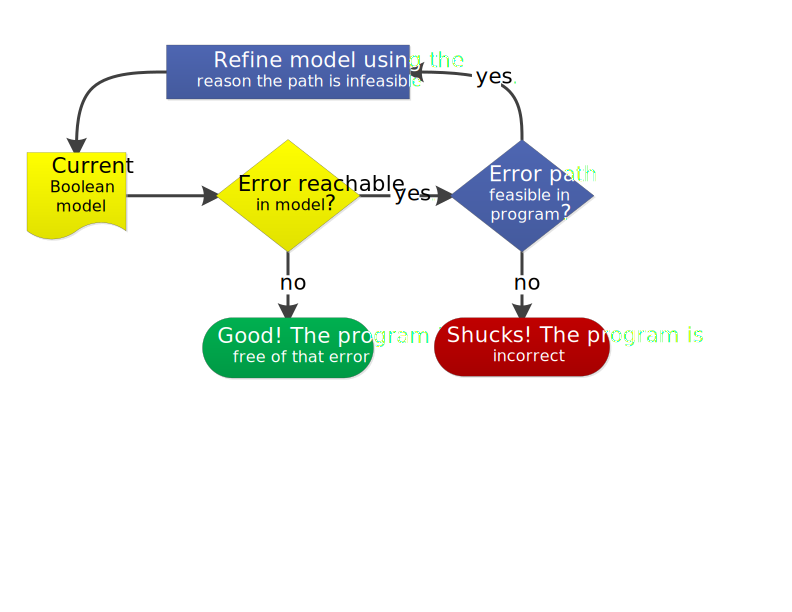
\includegraphics[width=0.75\textwidth]{images/cegar.pdf}
\end{center}

Basically what happens is the tool takes the original program and
produces an initial absraction as a Boolean program, which I will call
the ``model.'' The initial abstraction is very coarse, but it is
constructed to be \emph{sound} in the verification sense -- that is,
if an error state is unreachable in the model, it is guaranteed to be
unreachable in the original program. Whatever process is used to
generate Boolean programs must guarantee that each of the models it
produces is sound.

The CEGAR process then checks that initial abstraction to figure out
if there is an error in it, using the process we are about to
describe. If not, the original program is proved to be free of that
kind of error because the model is sound.

Conversely, suppose that the error state is reachable in the model. In
this case, the error-reaching path through the Boolean program is
passed to another tool which looks to see whether that path is
feasible in the original program or whether it is an imprecision
introduced by the current abstraction. If the path is actually
feasible, it means we've found a bug in the original program, and our
analysis is complete.

The magic of the CEGAR loop happens in the remaining case: there is a
path to an assertion in the model but that path is an imprecision and
doesn't correspond to something actually executable in the original
program. In this case, the path feasibility check doesn't just say
``this path is not feasible'' but returns an explanation of
\emph{why}. That \emph{why} is turned into some additional predicates
that the Boolean program should track, which will increase the
precision. The model is \emph{refined} by adding these prediates as
well, and the new abstraction is checked for correctness starting the
cycle anew.

This process (though using different techniques to check the Boolean
programs) is the foundation of the SLAM tool from Microsoft
Research. This tool is able to check many properties of Windows device
drivers, and has since the release of Vista been a part of the
official Windows Driver Development Kit under the name Static Driver
Verifier (SDV). Getting a clean bill of health from the SDV is needed
for the Windows logo certification. 

Drivers are an attractive target for verification because they tend to
be relatively small, tend to not make heavy use of the heap, have many
well-defined properties to check, and are relatively important
(because bugs will bring down your whole system). From Microsoft's
perspective, drivers are an attractive target because if a third-party
driver blue-screens your system, Microsoft gets the blame anyway.
\end{sidebar}


\section{Transition Systems}
We can formalize the type of structure pictured in
\cref{fi:program-transition-graph} as something called a \emph{transition
  system}. The idea of a transition system is really quite simple:
it's a (possibly-infinite) collection of states along with a
\emph{transition relation} that describes how states are
related. Formally, a transition system is a pair $(S, \rightarrow)$
where $S$ is some set and $\rightarrow$ a binary relation on $S$:
$\rightarrow \subseteq S \times S$. (We will write $p \rightarrow q$
for $(p, q) \in \rightarrow$.) It can be visualized as a
possibly-infinite directed graph.

\begin{example}
An example of another transition system is defined by the $\lambda$
calculus. States in this transition system correspond to terms in the
$\lambda$ calculus in De Bruijn form, and the transition relation sets
$s \rightarrow t$ exactly when $t$ can be obtained from $s$ via a
$\beta$ reduction. (We use De Bruijn form so we can ignore $\alpha$
renamings, which don't change the ``meaning'' of a $\lambda$ term. Of
course, using ``normal'' $\lambda$ notation and including $\alpha$
renamings in the transition relation would also result in a perfectly
valid transition system, as wolud including $\eta$ reductions.)

The following diagram shows some portions of this transition system,
written in normal notation instead of De Bruijn for clarity:\\
\begin{center}
  \includegraphics[width=\textwidth]{images/lambda-system.pdf}
\end{center}

Starting from any term in this transition system can result in (1)
eventually reaching a normal form, (2) reaching a loop in the
transition system, or (3) reaching an infinite chain of transitions
that never reaches a normal form. All three cases are illustrated
above.
\end{example}

When modeling a Boolean program $B$, we will treat the semantics of
the program as a transition system where the states $S$ are the set of
possible configurations of the program $B$ and the transition relation
$\rightarrow$ is any state transition that respects the semantics of
the program $B$. Checking reachability of the \emph{transition system}
is then the same as checking reachability of the Boolean program; the
former basically just gives us a formalism for the latter which, as we
will see, will let us check reachability.

However, a program's transition system can be infinite because of
recursion (like \cref{fi:boolean-example-program}), and so we need a
finite representation. That is where pushdown systems come into play:
pushdown systems give us a way to represent some infinite transition
systems.

(\Cref{fi:program-transition-graph} illustrates an infinite transition
system borne out of \cref{fi:boolean-example-program}. That program
has the property that if execution reaches the infinite portion, then
it will never terminate, but this does not need to be the case: it is
possible to have a program with an infinite number of reachable states
but where from any configuration, a halting state is reachable.)


\section{Pushdown Systems}

A pushdown system is a way of describing a transition system where:
\begin{enumerate}

\item Every state can be written \Config{p}{s} where $p$ is a
  ``control location'' drawn from a finite set $P$ and $s$ is a stack
  of items drawn from a finite set $\Gamma$. (The name ``control
  location'' is misleading here for our purposes: when modeling a
  Boolean program, we will use the control location to hold
  information about the current valuation of global variables; the
  program's instruction pointer will still live at the top of the
  stack as before.)

\item To decide what states $q$ in the transition system are
  successors of a given state $p$ (i.e. $p \rightarrow q$), you need
  only look at and change (1) the control location in $p$ and (2) the
  top item in the $p$'s stack. The transition may push or pop items
  from the stack, though we restrict it from popping more than one
  item.
\end{enumerate}

If you are familiar with a pushdown automaton (PDA), a PDS is very
similar except there is no input tape or input character component of
the transitions. If you like, you can think of a PDS as exploring the
configuration space of a PDA when you have complete control over the
input.

The two above restrictions means that we can define a PDS as follows:

\begin{definition}
  A pushdown system (PDS) $\mathcal{P}$ is a triple $(P, \Gamma,
  \Delta)$ where $P$ is a finite set (the ``control locations''),
  $\Gamma$ is also a finite set (the ``stack alphabet''), and $\Delta$
  is a set of rules of the form
  \Rule{\Config{p}{\gamma}}{\Config{q}{w}} where $p, q \in P$, $\gamma
  \in \Gamma$, and $w \in \Gamma^*$.
\end{definition}

A PDS describes a transition system in the following way. The set of
states in the transition system is the set of all configurations
\Config{p}{w} for $p \in P$ and $w \in \Gamma^*$. The transition
relation is defined as follows: $\Config{p}{\gamma\alpha} \rightarrow
\Config{q}{w\alpha}$ (with $\gamma \in \Gamma$ and $\alpha \in
\Gamma^*$) if and only if $\Rule{\Config{p}{\gamma}}{\Config{q}{w}}$
is a rule in the PDS. Basically, rule says that, if the transition
system is in control location $p$ and $\gamma$ is on the top of the
stack, then it can move to control location $q$, pop $\gamma$, and
push $w$. Hopefully this seems natural so far, especially if you're
familiar with PDAs.

Finally, to simplify the reachability algorithms (presented later), we
add one more restriction: every PDS rule must replace the top item on
the stack with either zero, one, or two other elements. (This is not a
fundamental restriction: it is possible to simulate any PDS without
this restriction by one with it, simply by adding new intermediate
states.) Rules are thus of one of the following forms:
\begin{itemize}
\item \Rule{\Config{p}{\gamma}}{\Config{p'}{\epsilon}} (which is called a
$\Delta_0$ rule)
\item \Rule{\Config{p}{\gamma}}{\Config{p'}{\gamma'}} (a $\Delta_1$
  rule)
\item \Rule{\Config{p}{\gamma}}{\Config{p'}{\gamma'\gamma''}} (a
  $\Delta_2$ rule)
\end{itemize}

(Note that it's $\Delta_1$ rules, not $\Delta_0$ rules, which leave
the stack height unchanged.)

We will be interested in two kinds of reachability questions: forward
reachability, called \poststar, and backward reachability, called
\prestar. In both cases, we ask what is reachable from a starting set
of configurations $C$, and the answer will be the set of reachable (or
reaching) configurations. The definitions are as follows:
\begin{itemize}
\item $\poststar_{\mathcal{P}}(C) = \{p' \mid \exists p\in C. p \rightarrow^*
  p'\}$x
\item $\prestar_{\mathcal{P}}(C) = \{p \mid \exists p'\in C. p \rightarrow^*
  p'\}$
\end{itemize}
In both cases, $\rightarrow^*$ is the reflexive transitive closure of
the transition relation defined by the PDS $\mathcal{P}$. I'll also
abuse notation and use $\poststar(p)$ to mean $\poststar(\{p\})$ for a
single configuration $p$, and similarly for \prestar.

\begin{center}
  \includegraphics[width=0.5\textwidth]{images/post-pre.pdf}
\end{center}

Reachability questions can then be expressed in two ways: if we want
to know whether a configuration $p'$ is reachable from a configuration
$p$, we can ask whether $p' \in \poststar(p)$ or whether $p \in
\prestar(p')$. (In the case of modeling Boolean programs, $p$ will
typically be the starting configuration (or the set of starting
configurations) and $p'$ will be the error configuration (or set of
error configurations).

By expressing a transition system as a PDS we have solved the problem
of having to finitely represent an infinite transition system, but we
are not done: the input and output of both \prestar\ and
\poststar\ may themselves be infinite sets, and we need a way of
representing those sets in such a way that we can still compute
\prestar\ and \poststar. For instance, in
\cref{fi:program-transition-graph}, $\poststar(..)$ is infinite.

\subsection{Representing Sets of Configurations}

In order to represent a set of configurations symbolically (and
finitely), we will use a slightly-modified form of finite
automaton.

For a PDS $\mathcal{P}$, we will define a $\mathcal{P}$-automaton as
$(Q, \delta, F)$. $Q$ is a set of states, and must be a superset of
$P$ (the PDS's set of states); $\delta: Q \times \Gamma_\epsilon
\rightarrow \powerset{Q}$ is the transition function; $F$ is the set
of accepting states. The automaton's alphabet (for standard finite
automata, usually called $\Sigma$) is the same as the PDS's stack
alphabet $\Gamma$, plus $\epsilon$. I'll drop the $\mathcal{P}$
suffix of ``$\mathcal{P}$-automaton'' and just refer to it as an
automaton or configuration automaton.

A configuration automaton $\mathcal{A}$ accepts a configuration
\Config{p}{w} if $\mathcal{A}$ starts in its state $p$, follows
transitions according to $w$ (starting from the top of the stack), and
can end in an accepting state $f \in F$. (This is just like the
standard definition of acceptance in an FA except that the machine
starts in the configuration's state instead of one fixed start state
$q_0$, and the symbols it reads are from the configuration's stack,
top-to-bottom.)

For instance, the following atuomaton accepts the configuration
\Config{p}{abc}:\\
\begin{center}
  \includegraphics[width=0.75\textwidth]{images/p-abc.pdf}
\end{center}

In cases where I never need to refer to certain states, I'll omit
their names from the diagram:\\
\begin{center}
  \includegraphics[width=0.75\textwidth]{images/p-abc-nolabel.pdf}
\end{center}

$\mathcal{P}$-automata can, of course, represent either finite or
infinite sets of configurations of $\mathcal{P}$. However, not every
infinite set of configurations can be reprsented by a
$\mathcal{P}$-automaton, just like not every infinite set of normal
strings can be represented by a standard finite automaton. If a set of
configurations \emph{can} be represented, then we say that set is
``regular''.

An interesting and important fact is that for any PDS, both
$\poststar(C)$ and $\prestar(C)$ are regular if $C$ is
regular. Furthermore, given an automaton representation of $C$,
reachability queries can be computed by a simple precess on that
automaton. We will discuss the process for \poststar\ in the next
section, and \prestar\ in the following. Both algorithms have a
similar flavor; which is easier is a matter of some debate.


\subsection{The post* Algorithm}

To compute \prestar\ or \poststar\ on an automaton $\mathcal{A}$, we
follow one or more \emph{saturation rules}. A saturation rule tells
you to find a transition in the automaton and a rule in the PDS which
match on their state and stack symbol, and then add to $\mathcal{A}$
one or more other transitions if they are not already present. This
will hopfeully become clear momentarily.

Conceptually, you just check to see if there are any saturation rules
that can be applied; if there are, then you apply them, but if not,
the process is complete and the automaton now holds the set of
configurations that is the \poststar\ (or \prestar) of what you
started with. In an actual implementation, this process becomes guided
by a worklist; we will examine that after describing the saturation
rules for the two algorithms.


Let's look at our first post* saturation rule. Suppose our automaton
looks like this, in part: \\
\begin{center}
  \includegraphics[width=0.75\textwidth]{images/unweighted-post-delta-1-setup.pdf}
\end{center}



The squiggly bit on the right represents possibly a bunch of states
and transitions, but it could also be none at all. (In the extreme
case, the node labeled $n$ could be the same as $p$ in which case the
$\gamma$ transition is a self loop, and $p$ could be accepting.) Call
$L(n)$ be the set of strings accepted by $\mathcal{A}$ starting from
state $n$.

What does this mean? This means that a configuration is accepted by
this machine if it takes the form \Config{p}{\gamma\alpha}, where
$\alpha$ some string in $L(n)$.

Now consider the PDS rule
\Rule{\Config{p}{\gamma}}{\Config{p'}{\gamma'}}. This rule means that,
in the transition system defined by $\mathcal{P}$, a successor of
\Config{p}{\gamma\alpha} is \Config{p'}{\gamma'\alpha}. This means
that \Config{p'}{\gamma'\alpha} must be accepted by the post*
automaton.

What can we do to make this happen?

The answer is remarkably simple: we just add a transition
$\Trans{p'}{\gamma}{n}$:\\
\begin{center}
  \includegraphics[width=0.75\textwidth]{images/unweighted-post-delta-1-result.pdf}
\end{center}

In other words, we have our first saturation rule (we will have to
revise these rules later however, because of the presence of
$\epsilon$ transitions):

   If there is a PDS rule
   \Rule{\Config{p}{\gamma}}{\Config{p'}{\gamma'}} and a transition
   \Trans{p}{\gamma}{n}, add a new transition
   \Trans{p'}{\gamma'}{n}. ($p$, $p'$, and $n$ need not be distinct.)

OK. So now what should we do about $\Delta_0$ and $\Delta_2$ rules?
Before we go further, I encourage you to try to predict the saturation
rules for these.

Let's look at $\Delta_0$ first. This is actually very similar to the
$\Delta_1$ case we just did.

Consider the PDS rule
\Rule{\Config{p}{\gamma}}{\Config{p'}{\epsilon}}. This rule means that,
in the transition system defined by $\mathcal{P}$, a successor of
\Config{p}{\gamma\alpha} is \Config{p'}{\alpha}, and the latter
configuration must be accepted by the post* automaton.

To make this happen, we just add a transition like last time except
this time we make in an $\epsilon$ transition:
$\Trans{p'}{\gamma}{n}$.\\
\begin{center}
  \includegraphics[width=0.75\textwidth]{images/unweighted-post-delta-0-result.pdf}
\end{center}


Formally, we have the following rule:

   If there is a PDS rule
   \Rule{\Config{p}{\gamma}}{\Config{p'}{\epsilon}} and a transition
   \Trans{p}{\gamma}{n}, add a new transition
   \Trans{p'}{\epsilon}{n}.

(We'll come back to this rule again in a moment -- it is not yet
complete.)

Finally, consider the $\Delta_2$ rule
\Rule{\Config{p}{\gamma}}{\Config{p'}{\gamma'\gamma''}}. This rule
means that, in the transition system defined by $\mathcal{P}$, a
successor of \Config{p}{\gamma\alpha} is
\Config{p'}{\gamma'\gamma''\alpha}. This means that
\Config{p'}{\gamma'\gamma''\alpha} must be accepted by the post*
automaton.

This one is a bit more complicated, because we have to add \emph{two}
transitions. But what should be the intermediate state? For reasons
which we will describe later, we add one new state for each
$(p',\gamma')$ pair; we will call this state $q_{p',\gamma'}$.

Thus the automaton picture looks as follows:
\begin{center}
  \includegraphics[width=0.75\textwidth]{images/unweighted-post-delta-2-result.pdf}
\end{center}

And we have the saturation rule

   If there is a PDS rule
   \Rule{\Config{p}{\gamma}}{\Config{p'}{\gamma'\gamma''}} and a
   transition \Trans{p}{\gamma}{n}, add new transitions
   \Trans{p'}{\gamma'}{q_{p',\gamma'}} and
   \Trans{q_{p',\gamma'}}{\gamma''}{n}, adding the state $q_{p',\gamma'}$
   if necessary.


\subsubsection{Correcting our \poststar\ saturation rules for $\epsilon$
  transitions}

Unfortunately, the saturation rules in the preceeding section are not
yet completely correct. To illustrate the problem, consider a PDS with
the following rules:

\begin{verbatim}
   p A -> p B C
   p B -> p eps
   p C -> p D
\end{verbatim}

By applying each of these rules in order, we see that the
configuration \Config{p}{D} is in $\poststar(\Config{p}{A})$.

However, let's apply the saturation rules exactly as given above,
starting from an automaton that accepts just the configuration
\Config{p}{A}. (Try this yourself before reading on!)

We start with
\begin{center}
  \includegraphics[width=0.75\textwidth]{images/epsilon-needed-0.pdf}
\end{center}

then apply the $\Delta_2$ saturation rule because we have a PDS rule
\Rule{\Config{p}{A}}{\Rule{p}{B C}} and a transition \Trans{p}{A}{f},
and get this:
\begin{center}
  \includegraphics[width=0.75\textwidth]{images/epsilon-needed-1.pdf}
\end{center}

then we apply the $\Delta_0$ saturation rule because we have a PDS
rule \Rule{\Config{p}{B}}{\Config{p}{\epsilon}} and a transition
\Trans{p}{B}{q_{p,B}}, and arrive at:
\begin{center}
  \includegraphics[width=0.75\textwidth]{images/epsilon-needed-2.pdf}
\end{center}

You might hope that we can now apply the $\Delta_1$ transition rule
with the PDS rule \Rule{\Config{p}{C}}{\Config{p}{D}}, but as written
it does not apply: there is no transition starting at $p$ with symbol
$C$. In fact, there is no additional steps we can take: the automaton
has reached saturation according to the preceeding rules.

Of course, the problem is that there's a \emph{path} that starts at
$p$ and begins by reading $C$, but that path starts with an $\epsilon$
transition.

(Note: a similar situation can arise with the $\epsilon$ transition on
the ``other side'' of the transition we're interested in, but only if
the initial query automaton has certain structures.)

We can handle this situation in two ways. The first is we modify our
three saturation rules so that they look for \emph{paths} rather than
just single transitions. If we use the notation \epspath{p}{\gamma}{n}
to mean a path with (optionally) some $\epsilon$ transitions, then a
$\gamma$ transition, then (optionally) some more $\epsilon$ transitions,
then our revised rules are:


   If there is a PDS rule
   \Rule{\Config{p}{\gamma}}{\Config{p'}{\gamma'}} and a path
   \epspath{p}{\gamma}{n}, add a new transition
   \Trans{p'}{\gamma'}{n}. ($p$, $p'$, and $n$ need not be distinct.)

   If there is a PDS rule
   \Rule{\Config{p}{\gamma}}{\Config{p'}{\epsilon}} and a path
   \epspath{p}{\gamma}{n}, add a new transition
   \Trans{p'}{\epsilon}{n}.

   If there is a PDS rule
   \Rule{\Config{p}{\gamma}}{\Config{p'}{\gamma'\gamma''}} and a path
   \epspath{p}{\gamma}{n}, add new transitions
   \Trans{p'}{\gamma'}{q_{p',\gamma'}} and
   \Trans{q_{p',\gamma'}}{\gamma''}{n}, adding the state
   $q_{p',\gamma'}$ if necessary.


The other option is to perform on-the-fly $\epsilon$ closure. We'll
leave the $\epsilon$ transitions in-place, but just ensure that we'll
never need to use them. To do this, we add one more rule:

    If there is a transition \Trans{q}{\epsilon}{q'} and
    \Trans{q'}{\sigma}{q''} (where $\sigma$ can either be a stack
    symbol in $\Gamma$ or $\epsilon$), add the transition
    \Trans{q}{\sigma}{q''}.


\subsubsection{The extra state in $\Delta_2$ rules.}

In this section we will attempt to explain the intuition behind the
behavior of the state added when dealing with $\Delta_2$ rules.  In
particular, we want to answer (1) why do we have to ``combine'' states
to begin with (we'll see what we mean by that), (2) why can we combine
the states that we do, and (3) why don't we combine more. These three
observations together suggest that the approach stated above, where we
add a $q_{p,\gamma}$ for each control location $p$ and stack symbol
$\gamma$, is correct, though I'm not claiming that this constitutes a
proof.

\subsubsubsection{Why do we have to combine states?}

Consider the PDS with the following rule:

  \Rule{\Config{p}{a}}{\Config{p}{ab}}

Starting from the configuration $c = \Config{p}{a}$, it is hopefully
clear that $\poststar(\{c\})$ should be the set of configurations of
the form \Config{p}{ab*}. (That is, the stack top is $a$ and under it
is any number of $b$s.)

Let's see what happens if we use a different $\Delta_2$ saturation
rule -- one that at first glance seems like it could be reasonable,
and you might have thought of -- so that it will \emph{always} add a
new state. For simplicity's sake, I'll use the version that ignores
$\epsilon$ transitions, but of course we still need to handle that
somehow. Stated formally:

   If there is a PDS rule
   \Rule{\Config{p}{\gamma}}{\Config{p'}{\gamma'\gamma''}} and a
   transition \Trans{p}{\gamma}{n}, add a fresh state $q$ then add
   transitions \Trans{p'}{\gamma'}{q} and \Trans{q}{\gamma''}{n}.

Runnng \poststar\ with this rule gives the following. We start with the
query automaton that represents $\{c\}$:
\begin{center}
  \includegraphics[width=0.75\textwidth]{images/mid-state-0.pdf}
\end{center}

Then apply the $\Delta_2$ saturation rule:
\begin{center}
  \includegraphics[width=0.75\textwidth]{images/mid-state-1.pdf}
\end{center}

Then apply the $\Delta_2$ saturation rule again:
\begin{center}
  \includegraphics[width=0.75\textwidth]{images/mid-state-2.pdf}
\end{center}

And again:
\begin{center}
  \includegraphics[width=0.75\textwidth]{images/mid-state-3.pdf}
\end{center}

You see the problem.

If we want \poststar\ to terminate, we want to be able to avoid adding
this chain of fresh states. The approach we'll take is to
\emph{combine} all of these states -- combine states with a common
source and symbol. So we take all of the states in the dotted region
and combine it into one:
\begin{center}
  \includegraphics[width=0.75\textwidth]{images/mid-state-combine.pdf}
\end{center}


Note that the self-loop on $q_{p,a}$ is present because there are
transitions from one $q$ to another $q$ in the expanded
version. Furthermore, note that this is the same automaton we get if
we apply the correct $\Delta_2$ saturation rule twice, at which point
we have reached saturation:
\begin{center}
  \includegraphics[width=0.75\textwidth]{images/mid-state-correct.pdf}
\end{center}
(On the second application, $n$ and $q_{p,a}$ are the same state,
which is why adding a transition from $q_{p,a}$ to $n$ adds a self
loop.)


\subsubsubsection{Why can we combine these states?}

Take the same PDS as before, but add a rule to it:

    \Rule{\Config{p}{a}}{\Config{p}{c}}

and then take our partially-done expanded post* automaton:
\begin{center}
  \includegraphics[width=0.75\textwidth]{images/mid-state-3.pdf}
\end{center}

Now what can we do? Well, we can run our $\Delta_1$ saturation rule
and add the following transitions:
\begin{center}
  \includegraphics[width=0.75\textwidth]{images/mid-state-with-c.pdf}
\end{center}


An interesting fact emerges. Every transition we added before to one
of our fresh states will prompt us to add the same \emph{additional}
transitions (just to each respective state). Call these transitions
$T$.  Furthermore, because we only ever add transitions starting from
a $p$ state (except when first creating a new fresh state), every
accepting path that traverses the fresh states at all will take one
transition in $T$ then follow the ``spine'' of fresh states to the
end. Finally, every transition along the spine will have the same
label because they were all added as the second transition when
looking at the same $\Delta_2$ rule, so the language this set of paths
accepts consists of one symbol that appears on an edge from $p$ to any
mid state, followed by zero or more symbols of what appears on the
spine transitions.

But we can express that language in a different way: we can collapse
all the fresh states into one, adding a self loop, and this gives us
the correct result.

\subsubsubsection{Why can't we combine more?}

You just can't.

I don't have as convincing an argument to make here; just it doesn't
make sense to combine states with a different control location, or a
different stack symbol.


\subsection{The \prestar\ algorithm}

Now that we've looked at \poststar, let's look at \prestar. In many
ways this is simpler: the presentation below (in accordance with the
literature) will present just one saturation rule for any PDS rule
\Rule{\Config{p}{\gamma}}{\Config{p}{w}} ($w \in \Gamma^*$), but why
that rule works is silghtly harder to think about because we are so
used to thinking about how program execution will proceed forwards.

Before continuing, try to deduce the saturation rule yourself:
remember that our goal is to produce an automaton that expresses the
set of configurations \emph{from} which a configuration in the
original query automaton is reachable. (If it is easier to think
about, feel free to state separate saturation rules for $\Delta_0$,
$\Delta_1$, and $\Delta_2$ PDS rules as we did for \poststar.)

Let's think through what we want in a similar way as before. Suppose
that we have a configuration $c = \Config{p}{w}$ that is represented
by our current automaton. We want to add some backwards-reachable
configurations. Well, how did the transition system get to $c$? If the
PDS has a rule \Rule{\Config{p'}{\gamma}}{\Config{p}{w'}} where $w'$
is a prefix of $w$ (let $w = w'w''$), that gives us one possible way:
we start in the configuration \Config{p'}{\gamma w''}, apply that
rule, then arrive in $\Config{p'}{w'w''} = c$.

How does this look in the automaton world? If $c$ is accepted by the
current automaton, then there's a series of transitions out of $p$
labeled with each symbol in $w'w''$:
\begin{center}
  \includegraphics[width=0.75\textwidth]{images/unweighted-pre-setup.pdf}
\end{center}

To accept \Config{p'}{\gamma w''}, we just need to add a $\gamma$
transition from $p'$ to the point at which the automaton has skipped
over $w'$. Graphically:
\begin{center}
  \includegraphics[width=0.75\textwidth]{images/unweighted-pre-result.pdf}
\end{center}

(For $\Delta_0$ rules, this saturation rule will result in us adding a
self-loop on a $p$ state.)  Note that this rule works no matter the
length of $w'$; but we still always just add a single transition, and
there is no need for any new mid states.

That's all there is to it.


\section{From Unweighted to Weighted PDSs}

Above we described pushdown systems from the perspective of doing
model checking -- it is explicitly exploring the state space of a
program. Even when paired with something like SLAM, which is doing
iterative refinement of a ``real'' program, we are still doing
explicit-state model checking of the current Boolean program model.

Practically speaking it can be useful to think about WPDSs in a bit
different terms. While they \emph{are} a way of defining a weighted
transition system with weights from some bounded idempotent blah blah
blah, what they are usually used for is essentially dataflow analysis
(abstract interpretation) over some program. I'll try to describe
things in those terms. In the final section, I'll try to relate that
picture to the somewhat more abstract presentation in the literature.

Finally, one notion that I didn't get right away when I was learning
is what is meant by \emph{weight}. What I think you should probably
\emph{not} have as a model in your mind is something like a weighted
graph from when you were learning graph theory in your algo class,
which you might run some weighted shortest path problem on. This
picture has enough truth in it that I can't say it is \emph{completely
  incorrect}\footnotemark, but if that's all you know it's very
misleading. Weights in general are a much more abstract notion; as
you'll see momentarily, in our setting, they will represent abstract
transformers. To address the issue of unhelpful preconceptions, for
the time being, you may find it useful to pretend that WPDSs are
instead called ``dataflow pushdown systems'' and mentally substitute
``dataflow transformer'' where I say ``weight''.

\footnotetext{Weights in the sense of an typical algorithms course are
  a specific instance of these more general weights, and many
  traditional algorithms on weighted graphs like Dijkstra's algorithm
  have corresponding generalized versions. Sometimes the literature
  will even discuss these generalized versions calling them ``shortest
  path'' problems, but they'll still be using the generalized
  weights.}

In the following, I assume you know about dataflow analysis (or
abstract interpretation).

\subsection{Weights for dataflow analysis and the MOAVP goals}

Consider some typical dataflow analysis. There's some domain $D$ of
possible dataflow facts (e.g. $\powerset(vars \times \bbN_\bot^\top)$
for constant propagation and a ``meet'' ($\meet$) that is used to
combine dataflow facts when paths in the program converge\footnote{In
  this paper, I approach things using dataflow analysis terms
  rather than abstract interpretation: $\bot$ represents ``anything is
  possible'' and $\meet$ is used to combine the values of two paths.}.
When propagating information ``through'' a basic block $b$, you use
some transformer $\tau_b: D \rightarrow D$ to translate the dataflow
fact before the block to the one after the block, or vice versa
(depending on whether you're doing a forwards or backwards
analysis). The goal is to find the ``meet over all valid paths''
solution from the program's start to its finish\footnote{I'll discuss
  WPDSs as if they're actually computing the MOAVP solution to a data
  flow problem, but really this is only true if the dataflow problem
  is distributive -- that is, $(a \extend b) \combine (a \extend c) =
  a \extend (b \combine c)$ and similarly for the right-hand side. In
  dataflow terms, this says that instead of looking at the
  (possibly-infinite) set of paths from start to finish, computing the
  dataflow transformers across that path, then combining the results
  from the different paths, we can instead combine the results ``as we
  go along'', at places where paths come together.}.

If you're familiar with ``meet over all paths'' but not ``valid
paths'', a ``valid path'' is one where control does not use some call
site $c$ to call a function \Code{foo} but then return to a different
call site. This is what gives us context sensitivity. The following
diagram illustrates:

When doing dataflow analysis with a WPDS, we actually treat the set of
transformers $\tau_b$ explicitly. Our \emph{weight domain} then
consists of the set of these transformers and their compositions, and
some operations on them. We need two operations, and both are pretty
familiar.

The first opreation is composition. If we take some path through the
program where the transformers are $\tau_1$, $\tau_2$, and $\tau_3$,
then a transformer that represents the net effect of the path is just
$\tau_3 \circ \tau_2 \circ \tau_1$. Note, however, how using $\circ$
``reverses'' the path; i.e. the transformer that was used last appears
first when we write it out. This is inconvenient, so we invent a
``reversed composition'' operator. Since I have to make something up
anyway, I'll match the usual WPDS literature and use $\tau_1 \extend
\tau_2 \extend \tau_3$ for $\tau_3 \circ \tau_2 \circ \tau_1$. We
pronounce $\extend$ as ``extend'', but really it's just function
composition in our setting.

The second operation is meet, $\meet$. We know how to meet two data
values $d_1$ and $d_2$, but not necessarily transformers. But it's
pretty simple: $\tau_1 \meet \tau_2$ is going to be a new function
defined as follows: $(\tau_1 \meet \tau_2)(d) = (\tau_1(d)) \meet
(\tau_2(d))$. In other words, the meet of two functions takes its
argument, applies each of the two functions individually, then meets
the result.

Finally, we also have available two constant transformers: $\Zero$ and
$\One$. $\Zero$ is a transformer which essentially means
``impossible'': if a path has weight $\Zero$, then it is an infeasible
path according to the abstraction. It has the property that $\Zero
\extend x = x \extend \Zero = \Zero$ and $\Zero \combine x = x
\combine \Zero = x$ for all dataflow elements (transformers)
$x$. $\Zero$ is like the $\top$ element from the original datalow
domain. $\One$ is the identity transformer: $\One \extend x = x
\extend \One = x$ holds for all $x$.

This gives us the elements we'll need for our weight domain. 

When computing a forwards-flow analysis then, what our goal is as
follows:
\begin{itemize}
\item For each program point $p$
  \begin{itemize}
    \item paths = \{all valid paths from start to $p$\}
    \item label $p$ with meet(paths)
  \end{itemize}
\end{itemize}
This labels each point $p$ with an aggregate transformer that
represents all possible ways of starting from the initial state and
getting to $p$. We can then apply that transformer to the starting
dataflow fact to obtain the dataflow fact that holds at
$p$. Forwards-flow problems will be computed with weighted \poststar.

When computing a backwards flow analysis, the goal is similar:
\begin{itemize}
\item For each program point $p$
  \begin{itemize}
    \item paths = \{all valid paths from $p$ to finish\}
    \item label $p$ with meet(paths)
  \end{itemize}
\end{itemize}
This labels each point with an aggregate transformer that represents
all possible ways of getting from that point to the end of the
program. Backwards-flow problems will be computed with weighted
\prestar.

Both of these problems generalize. We can start from any regular set
of configurations instead of just a single start node, or end in any
regular set of configurations. For instance, we could ask about
configurations where we specify not just a program point but also a
set of possible stacks: perhaps we are only interested in a point $p$
if \Code{foo} is somewhere on the stack.  Such \emph{stack-qualified
  queries} are a strict increase in power of WPDSs relative to other
methods for context-sensitive analysis, such as Shriri-Pnuelli's
framework.


\subsection{Creating a WPDS model of a program}

TODO


\subsection{Representing weighted configuration sets}

We will represent sets of weighted configurations in almost the same
way as before. However, instead our slight modification to standard
finite automata, we will use a \emph{weighted} FA (WFA). Structurally,
this just means that each transition is annotated with a
weight\footnotemark. (Later we'll add weights to states as well.)

Unfortunately, the interpretation of these WFAs differs slightly
between \prestar\ and \poststar, as described next. The differences
are not as strange or deep as they appear like they may be initially
however, and we explore a deeper connection.

\subsubsection{Interpreting the result of \prestar}
For \prestar, the interpretation is still pretty simple. In the unweighted
case, a path from an initial state $p$ to an accepting state with
$\gamma_1\gamma_2\dots\gamma_n$ as the edge symbols indicates that the
configuration $c = \Config{p}{\gamma_1\gamma_2\dots\gamma_n}$ is
contained within the set in question. In the weighted case, it
indicates that $c$ is accepted \emph{with weight} $w_1 \extend w_2
\extend \dots \extend w_n$, where $w_i$ is the weight on the
transition that corresponds to $\gamma_i$.

Actually, the previous sentence is a lie. What it \emph{really} means
is that there is \emph{some set of paths} in the WPDS's transition
system for which the meet of the weights of those paths is $w_1
\extend w_2 \extend \dots \extend w_n$ -- but there may be other paths
in the transition system whose weights are not incorporated in $w_1
\extend w_2 \extend \dots \extend w_n$. This can occur if
\emph{automaton} has multiple paths that accept the same
configuration. (Don't get paths through the WPDS's transition system
confused with paths through the automaton!) In such a case, to get the
MOAVP solution of the transition system, we need to look at every
corresponding path in the \emph{automaton}, take its weight, then take
the meet of all of those.

For example:

\subsubsection{Interpreting the result of \poststar}

Interpreting the weights of the \poststar\ automaton is a bit
different. Most things stay the same regarding what paths through the
WFA we look at and such, but computing the weight of a path is the
opposite. Here's the rule: the weight of a path $\gamma_1 \gamma_2
\dots \gamma_n$ is $w_n \extend \dots \extend w_2 \extend w_1$ (with
$w_i$ being the weight on the transition with symbol $\gamma_i$, as
before). In other words, it's the reverse of before\footnotemark.

\footnotetext{In a bit of irony this means we could revert to using
  $\circ$ instead of $\extend$, then write it in forward
  order. However, I'll stick with $\extend$ to match the existing
  literature.}

Why is it the reverse? Well, I'll come back to that topic in a
bit. First we will need to reexamine the interpretation of the
\prestar\ automaton.

\subsubsection{Interpretations of the automaton, unified (somewhat)}

Let's express the interpretation of the \prestar\ automaton (i.e. the
result of running \prestar) in a different manner. This may seem a
little strange for a moment, but hopefully you'll find the explanation
useful.

Consider what the meaning of ...


You can kind of think of following a path in the \prestar\ automaton
in the following way. Suppose you are given a WPDS configuration
$c=\Config{p}{\gamma}$, and want to determine whether that
configuration is accepted by the WFA. We can think of starting in the
WFA state $p$, then successively popping off the top symbol of
$\gamma$ while following the corresponding WFA transition. When we've
popped off all of the symbols in $\gamma$, if the WFA is in an
accepting state then it means that configuration is accepted.

Expounding on this idea, if we want to explore the reachability space
of a WPDS $\mathcal{P}$ from some initial set of configurations, we
put the WPDS into any of the starting configurations, ``run'' 

-- something missing about why PA makes sense --

Interpretation of the \poststar\ automaton is a bit different. Because
\poststar\ and \prestar\ are opposites, we have to do the opposite thing:
Instead of running the WPDS then the WFA, we will do the opposite, and
run the WFA followed by the WPDS. We also think of the interpretation
of the WFA in the opposite: Instead of saying that a configuration is
accepted if we can pop it off using WFA transitions, we'll say it's
accepted if we can start with an empty stack and \emph{push} symbols
to get the stack in question (pushing a symbol for each WFA
transition).

But there's something funky here: a path with symbols $\gamma_1
\gamma_2 \dots \gamma_n$ will, if we just push the symbols in
sequence, give us the stack $\gamma_n \dots \gamma_2 \gamma_1$, with
$\gamma_n$ at the top of the stack. This isn't the interpretation we
meant: transitions out of the initial states should be the start
symbols. To get at the stack with $\gamma_1$ at the top, we need to
start at the other end -- in other words, we need to push the symbols
in the \emph{reverse order} of the path we accept them.

(Note that if we ignore weights, we haven't changed anything from the
unweighted post* case! If we want to know if a configuration is
accepted regardless of its weight\footnotemark, we still follow
transitions starting from the top of the stack, same as before. The
reversal of the path argument has to deal with how the weights are
built up only.)

The fact that we conceptually pushed $\gamma_n$ first means that we've
arrived at our rule: the \emph{weight} of a path $\gamma_1 \gamma_2
\dots \gamma_n$ is actually $\gamma_n \extend \dots \extend \gamma_2
\extend \gamma_1$.





\footnotetext{One caveat: if a configuration has the weight $\top$
  it's reasonable to say that is unreachable. If no transitions in the
  query automaton and no WPDS rules have weight $\top$ however, this
  will never arise.}


\subsection{Putting it all together}

What we are eventually interested in is the set of dataflow
values that can arise at a program point $n$. This corresponds to
multiple possible configurations -- and we want the meet of the weight
of each of those configurations. This leads to the following, naive,
algorithm for doing forwards-flow dataflow analyses:
    - Set up a query automaton from the initial configuration(s)
    - Run post*
    - For each prgoram point $n$
          - $w_{all} = \top$
          - For \emph{every path} $p$ that starts with $n$ from an
            initial state to an accepting state
              - Let $w$ be the weight of the path (using $\extend$),
                remembering that we are extending in reverse
              - $w_{all} = w_{all} \meet w$
          - Label $n$ with $w_{all}$

Later we'll look at getting rid of that explicit ``look at all
paths.''

The corresponding algorithm backwards-flow analysis is similar, but
this is a complication. There can be configurations in the pre*
automaton that are not actually reachable from the initial state. For
instance, if we run pre* on the example from section blah (from the
program's exit state with no stack), we get the following automaton:

This automaton accepts configurations like \Config{p}{foo_3 main_3}
where $main_3$ isn't a call site!

This configuration doesn't make sense as far as the program's
semantics are concerned, but the WPDS's transition system doesn't know
that. As far as the transition system is concerned, if it starts in
the configuration \Config{p}{foo_3 main_3}, then it can get to the
final state -- and indeed this is the case. 

So what we want to do is simple conceptually. We will run an
\emph{unweighted} post* from the set of initial configurations, then
intersect the result with our WFA from pre*. (WFA intersection
proceeds as normal FA intersection, except that weights are computed
in the resulting automaton by ???.) We then examine *this* automaton.

  The reason this didn't come up in the unweighted case is that we
  were asking a different question. At first glance we'd still have
  the same problem, since the unweighted pre* automaton would still
  accept that configuration. However, in the unweighted case we'd just
  ask whether a particular configuration (or any of a set of
  configurations) is accepted. Assuming our configuration of interest
  isn't one of these infeasible configurations, their presence doesn't
  matter.
  
  The problem comes from the fact that now we want to get the dataflow
  fact for some node $n$, and we do it by looking at all of the paths
  in the WFA that start with $n$. But now the presence of infeasible
  paths matters, because we want to exclude them.

So here is the process of carring out a backwards dataflow problem:
\begin{verbatim}
    - C_end = query automaton for exit configuration(s)
    - a_pre = pre(C_end)
    - C_start = query automaton for starting configuration(s)
    - a_post = post(C_start)
    - answer = a_pre \cap a_post
    - For each prgoram point $n$
          - $w_{all} = \top$
          - For \emph{every path} $p$ in answer that starts with $n$
            from an initial state to an accepting state
              - Let $w$ be the weight of the path (using $\extend$,
                remembering we are extending ``forward'')
              - $w_{all} = w_{all} \meet w$
          - Label $n$ with $w_{all}$
\end{verbatim}

\subsection{Weighted post*}

Finally, we have to discuss how to carry out the post* and pre*
algorithms. We'll start with post*.

The general idea of both algorithms is very similar to the unweighted
case. Really the only difference is we will change each rule from
something of the form ``look for a PDS rule and FA transition blah
blah and add a new transition blah blah'' and turn it into ``look for
blah blah and \emph{update the weight on transition} blah blah''
(instead of just adding it). We run the saturation rules until not
only are there no new transitions that are necessary but until no rule
will change any weight.

So let's look at the $\Delta_1$ case. The unweighted rule was

   If there is a PDS rule
   \Rule{\Config{p}{\gamma}}{\Config{p'}{\gamma'}} and a transition
   \Trans{p}{\gamma}{n}, add a new transition
   \Trans{p'}{\gamma'}{n}. ($p$, $p'$, and $n$ need not be distinct.)

Let's look at what it means in the weighted case. Suppose that the
weight of the PDS rule is $w_r$, the weight of the transition
\Trans{p}{\gamma}{n} is $w_t$, and the weight of the transition
\Trans{p'}{\gamma'}{n} is currently $w$. If the latter transition does
not yet exist, then we'll set $w = \top$. (Remember, $\top \meet x =
x$. It essentially reflects an impossible weight.) Conceptually, you
can think of \emph{every} transition being initially present in the
automaton but with weight $\top$, though you have to revise some other
explanations in light of this.

Here's a diagram of the transition system and the WFA:

Suppose we have some path $\pi$ in the WFA that starts at $n$ and
leads to an accepting state, and that path has weight $w_\pi$. (And
for sake of simplicity of the explanation, suppose there is only one
path with $\pi$'s labels.)

// start eding here invalid markup
This means that it is possible to start in the transition system from some
  configuration in the query set and arrive at the configuration
  \Config{p}{\gamma \pi} while the MOAVP weight is $w_t \extend
  w_\pi$.\footnotemark
If we Similarly, the MOAVPs solution from the query set to
  \Config{p'}{\gamma'\pi} is $w_r \extend w_t \extend w_\pi$


\footnotetext{Really it's the meet of all MOAVPs solutions from
  anything in the query set: ....}

Here's a diagram of the transition system and the WFA:

If we suppose that this is the first time we're looking at this
$\Delta_1$ rule, there are at least two sets of possibilities for how
to get to the configuration \Config{p'}{\gamma'\pi}. Because
$\gamma'\pi$ was already accepted, whatever paths we found before is
one such set. The second way is what we just discovered: use one of
the ways to get to the configuration \Config{p}{\gamma \pi}, then the
PDS $\Delta_1$ rule we are looking at. Here is a picture:

We want the MOAVPs solution, so we need to take the meet of all of
these paths. The weight of the first set of paths is $w_{t'} \extend
w_\pi$.\footnotemark The weight of the second set of paths is $w_t
\extend w_\pi$ to get to \Config{p}{\gamma \pi} then the weiht of the
rule, giving $w_r \extend w_t \extend w_\pi$.

\footnotetext{Here and in the next moment we are using a fact which I
  haven't really told you, which is that $a \extend (b \meet c) = (a
  \extend b) \meet (a \extend c)$. This doesn't necessarily always
  hold -- but it must for WPDSs to work.}

This means that the new weight for \Config{p'}{\gamma' \pi} should be
$(w_{t'} \extend w_\pi) \meet (w_r \extend w_t \extend w_\pi)$ which
equals $(w_{t'} \meet (w_r \extend w_t)) \extend w_\pi$.

Note that we can achieve this (at least for this path) by updating
$w_{t'}$ to be $w_{t'} \meet (w_r \extend w_t)$. Furthermore, you can
repeat this argument for any other paths and configurations that would
be affected by this change, and find out that the same weight will
work out for each of them.

This gives our saturation rule:

   If there is a PDS rule
   \Rule{\Config{p}{\gamma}}{\Config{p'}{\gamma'}} with weight $w_r$,
   a transition \Trans{p}{\gamma}{n} with weight $w_t$, and a
   transition \Trans{p'}{\gamma'}{n} with weight $w_{t'}$, update the
   weight on the transition according to $w_{t'}' = w_{t'} \meet (w_r
   \extend w_t)$. If \Trans{p'}{\gamma'}{n} is not present, add it
   with weight $w_t \extend w_r$.

(Note that the case where it was not present will result in the same
   effect as treating it as being there but with weight $\top$. I
   won't include that final clause in the future.)

And here is a graphical picture of what it means:


We'll come back to $\Delta_0$ rules, but here's the $\Delta_2$
saturation rule:

   If there is a PDS rule
   \Rule{\Config{p}{\gamma}}{\Config{p'}{\gamma'\gamma''}} with weight
   $w_r$, a transition \Trans{p}{\gamma}{n} with weight $w_t$, and a
   transition \Trans{p'}{\gamma'}{q_{p',\gamma'}} with weight
   $w_{t'}$, then update $w_{t'}$ following $w_{t'}' = w_{t'} \meet
   (w_r \extend w_t)$. Finally, add the transition
   \Trans{q_{p',\gamma'}}{\gamma''}{n} with weight $\lambda x.x$ if it
   does not already exist.

Note that the transition outgoing from the state $q_{p',\gamma'}$ will
\emph{always} be $\lambda x. x$, as we only ever modify the weight of
transitions out of an initial state. (Though without seeing the
$\Delta_0$ saturation rule you won't know that for sure, of course.)

Here's a diagram:


Finally we have the rule for $\Delta_0$. We are going to weave
$\epsilon$ closure into this rule, so it is a bit more complicated
than the other rules we've seen.

The first part of the rule is what you might expect:

   If there is a PDS rule
   \Rule{\Config{p}{\gamma}}{\Config{p'}{\epsilon}} with weight $w_r$,
   a transition \Trans{p}{\gamma}{n} with weight $w_t$, and a
   transition \Trans{p'}{\epsilon}{n} with weight $w_{t'}$, update the
   weight on the transition according to $w_{t'}' = w_{t'} \meet (w_r
   \extend w_t)$.

And now we need to perform $\epsilon$ closure. The unweighted version
would continue:

   Now for any transition \Trans{n}{\sigma}{n'}, add a transition
   \Trans{p'}{\sigma}{n'}.

(Note that $\sigma$ may be $\epsilon$, in which case adding
\Trans{p'}{\sigma}{n'} will also give you more things to do with
this rule later.)

So what should the weight be on \Trans{p'}{\sigma}{n'}? Well, for
starters, if that transition is already present then it will already
have a weight $w_{t''}$, so we'll have to meet in that. (Whenever we
update a weight we always take the meet with the old version.) But
what's the new information we've discovered?

   Now for any transition \Trans{n}{\sigma}{n'} with weight $w_{t''}$,
   update the weight on the transition \Trans{p'}{\sigma}{n'}
   according to 





   If there is a PDS rule
   \Rule{\Config{p}{\gamma}}{\Config{p'}{\epsilon}} with weight $w_r$,
   a transition \Trans{p}{\gamma}{n} with weight $w_t$, and a
   transition \Trans{p'}{\epsilon}{n} with weight $w_{t'}$, ...



\end{document}
